\section{Real Data}
\label{sec:data}

We analyze a dataset that was collected to investigate the eating preferences of the wolf spider, genus \textit{Schizocosa}, towards the prey orders \textit{Diptera}, \textit{Collembola}.  Predators, caught in traps, were DNA sequenced to determine whether or not any \textit{Diptera} or \textit{Collembola} existed in the predators' guts for each time period.The left panel of figure~\ref{fig:gutP} plots the percentage of spiders that had the prey in their guts across time.  Prey were similarly collected, in traps distributed across the field site of interest {\color{red} where?}.  These data were collected for each month from October $2011$ to March $2013$.  On average, about $34$ and $69$ spiders and prey, respectively, were caught in each time period.  The range of the sample sizes, across all $18$ months, is $11$ to $181$ for caught spiders, and is from $24$ to $76$ for caught prey.  

\begin{figure}
  \centering
  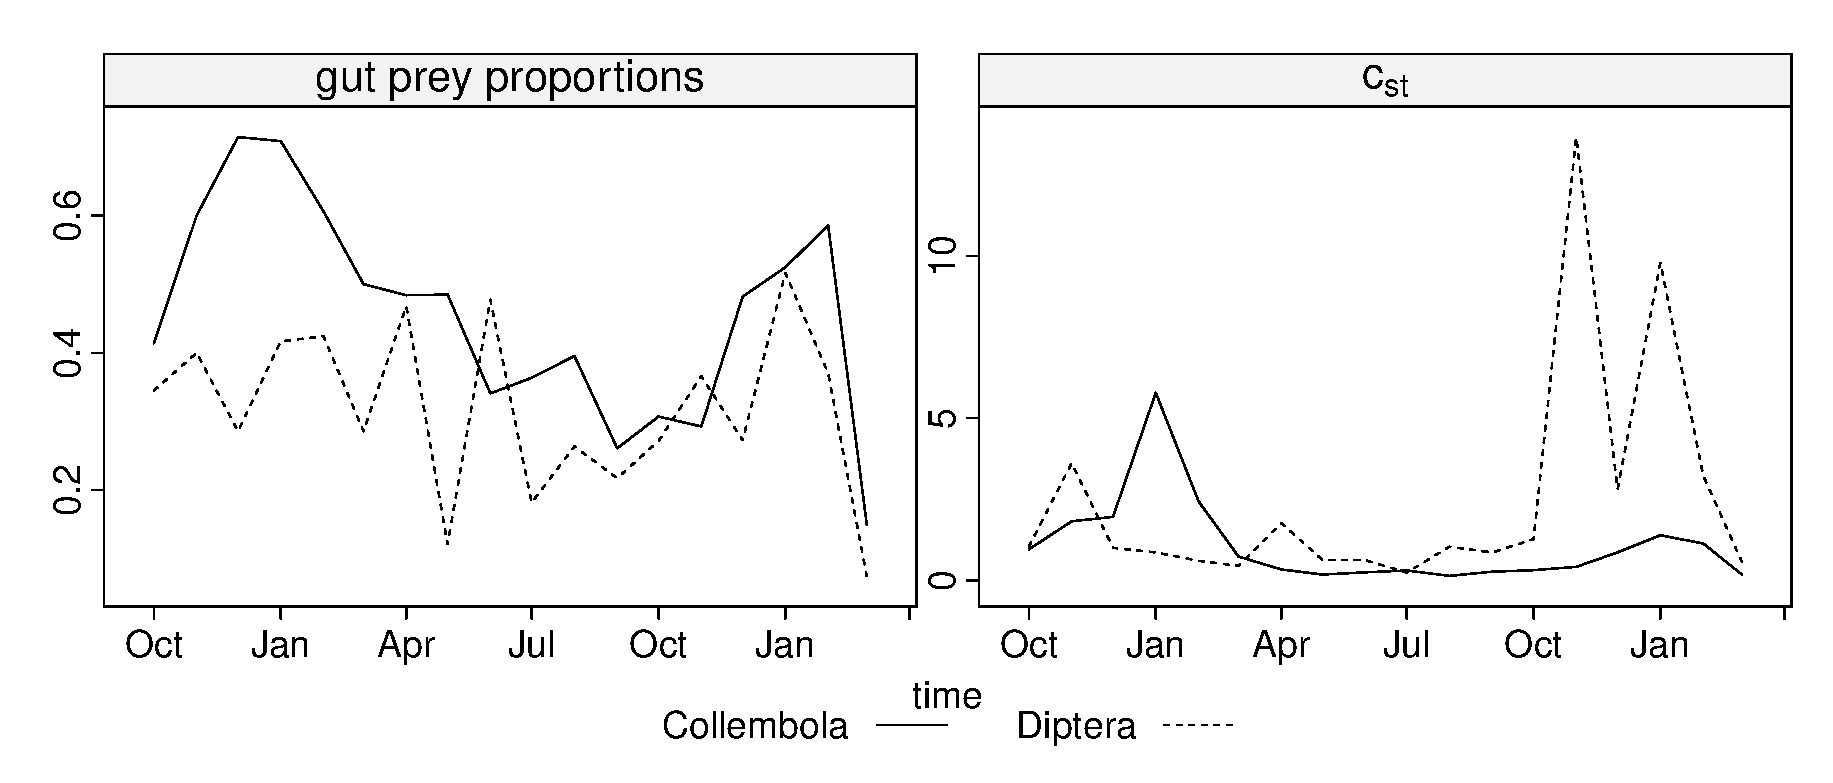
\includegraphics[scale=0.5]{time}
  \caption{moar words}
  \label{fig:gutP}
\end{figure}


 Following our hierarchy of hypotheses, we find that the most parameter rich model, $\lambda_{st} = c_{st} \gamma_{st}$ fits these data best.  This model estimates $72$ parameters in total; since, in this case, there are two prey of interest and $18$ time periods, it takes $36$ parameters to estimate each $c_{st}$ and $\gamma_{st}$.  The right panel of figure~\ref{fig:gutP} plots the points estimates of $c_{st}$ for both prey and across all time periods.  

With the model $c_{st}$ in mind, we can now test any number of linear contrasts.  Here, we test $c_{1t} = c_{2t}$, for $t \in \{1, \ldots, 18\}$.  Using a level of significance of $0.05$, and after making a Bonferroni multiple comparisons adjustment, we find that the two prey are similarly prefered in October, November, and December of $2011$ and for March and July of $2012$.  


%%% Local Variables: 
%%% mode: latex
%%% TeX-master: "main"
%%% End: 
